\documentclass[class=report,crop=false]{standalone}
\usepackage[screen]{../exo7book}

% Commande ponctuelle
\newcommand{\alenvers}[1]{\rotatebox[origin=c]{180}{#1}}
\newcommand{\vect}{\overrightarrow}

\begin{document}

%====================================================================
\chapitre{Calcul formel}
%====================================================================

%\insertvideo{ciw-QPp7p98}{partie 4. Suites récurrentes et visualisation}

%%%%%%%%%%%%%%%%%%%%%%%%%%%%%%%%%%%%%%%%%%%%%%%%%%%%%%%%%%%%%%%%
\setcounter{section}{3}
\section{Suites récurrentes et visualisation}

%--------------------------------------------------------
\subsection{Visualiser une suite récurrente}

\begin{tp}
Fixons $a\in\Rr$. Définissons une suite $(u_n)_{n\in\Nn}$ par récurrence :
$$u_0 = a \qquad \text{et} \qquad u_{n+1} = \exp(-u_n) \quad \text{pour } n\ge 0.$$
\begin{enumerate}
  \item Calculer les premiers valeurs de la suite pour $a=-1$. 
  \'Ecrire une fonction qui renvoie ces premières valeurs sous la forme d'une liste.
  
  \item Sur un même graphique tracer le graphe de la fonction de récurrence $f(x) = \exp(-x)$, la première bissectrice $(y=x)$
  et la trace de la suite récurrente, c'est-à-dire la ligne brisée 
  joignant les points $\big(u_k,f(u_k)\big)$, $(u_{k+1},u_{k+1})$ et $\big(u_{k+1},f(u_{k+1})\big)$.
 
  \item \'Emettre plusieurs conjectures : la suite ou certaines sous-suites sont-elles
  croissantes ou décroissantes ? Majorées ? Minorées ? Convergentes ?
  
  \item Prouver vos conjectures.
\end{enumerate}

\end{tp}
\begin{center}
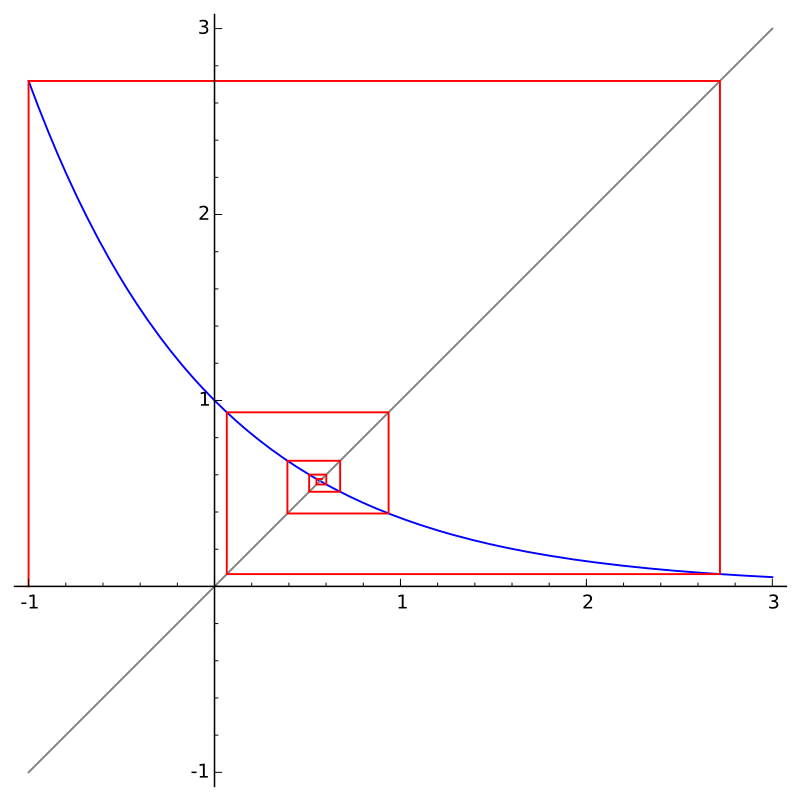
\includegraphics[scale=0.6]{figures/suites-visual1}
\end{center}

\begin{enumerate}
  \item 
On définit la fonction $f(x)=\exp(-x)$ par la commande \codeinline{f(x) = exp(-x)}.

\insertcode{algos/suites-visual-tex1.sage}{suites-visual.sage (1)}

Par exemple, la commande \codeinline{liste_suite(f,-1,4)}
calcule, pour $a=-1$, les $4$ premiers termes de la suite $(u_n)$ ;
on obtient la liste :

\centerline{\codeinline{[-1, e, e^(-e), e^(-e^(-e))]}}

correspondant aux termes : $u_0=-1$, $u_1 = e$,
$u_2 = e^{-e}$ et $u_3 = e^{-e^{-e}}$, où l'on note $e=\exp(1)$.

\item Nous allons maintenant calculer une liste de points.
On démarre du point initial $(u_0,0)$,
puis pour chaque rang on calcule deux points :
$\big(u_k,f(u_k)\big)$ et $\big(u_{k+1},u_{k+1}\big)$.
Notez que chaque élément de la liste est ici un couple $(x,y)$ de
coordonnées.

\insertcode{algos/suites-visual-tex2.sage}{suites-visual.sage (2)}


Par exemple, la commande \codeinline{liste_points(f,-1,3)}
calcule, pour $a=-1$, le point initial $(-1,0)$ et les $4$ premiers 
points de la visualisation de la suite $(u_n)$ par une ligne brisée ;
on obtient la liste :

\centerline{\codeinline{[(-1, 0), (-1, e), (e, e), (e, e^(-e)), (e^(-e), e^(-e))]}}
et il ne reste plus qu'à tracer le graphe des objets demandés.
% la fonction et construire
%la suite en traçant les segments reliant les points.

\insertcode{algos/suites-visual-tex3.sage}{suites-visual.sage (3)}

Par exemple, la figure illustrant ce tp est construite par la commande
\codeinline{dessine_suite(f,-1,10)}.

\bigskip

\item  (et 4.) Passons à la partie mathématique. Pour simplifier l'étude, nous allons supposer 
$a=-1$. Donc $u_0=-1$ et $u_1=f(u_0)=\exp(1) = e$.
\begin{enumerate}
  \item La fonction $f$ définie par $f(x)=\exp(-x)$ est décroissante.
  La fonction $g$ définie par $g(x) = f\big( f(x) \big)$ est donc croissante.
  
  \item La suite $(u_{2n})_{n\in\Nn}$ 
  des termes de rangs pairs est croissante. En effet :
  $u_2 = e^{-e} \ge -1= u_0$, puis 
  $u_4 = f \circ f( u_2 ) \ge f\circ f(u_0) = u_2$
  car $f\circ f=g$ est croissante.
  Par récurrence $u_6 = f \circ f (u_4) \ge f\circ f (u_2) = u_4$...
  La suite $(u_{2n})$ est croissante. 

  \item Comme $u_2 \ge u_0$ et que $f$ est décroissante alors $u_3 \le u_1$.
  On démontre alors de la même façon que la suite 
  $(u_{2n+1})_{n\in\Nn}$ des termes de rangs impairs est décroissante.
  
  \item Enfin, toujours par la même méthode et en partant de
  $u_0 \le u_1$, on prouve que $u_{2n} \le u_{2n+1}$.
  
  \item La situation est donc la suivante :
  $$u_0 \le u_2 \le \cdots \le u_{2n} \le \cdots \le u_{2n+1} \le \cdots \le u_3 \le u_1$$
  
  La suite $(u_{2n})$ est croissante et majorée par $u_1$, donc elle converge. Notons $\ell$
  sa limite.
  
  La suite $(u_{2n+1})$ est décroissante et minorée par $u_0$, donc elle converge. Notons $\ell'$
  sa limite.
  
  \item Par les théorèmes usuels d'analyse, la suite $(u_{2n})$
  converge vers un point fixe de la fonction $g=f \circ f$, 
  c'est-à-dire une valeur $x_0$ vérifiant $f\circ f(x_0)=x_0$.
  Une étude de la fonction $g$ (ou plus précisément de $g(x)-x$) montrerait que $g$
  n'a qu'un seul point fixe. Voici le graphe de $g$.
  \begin{center}
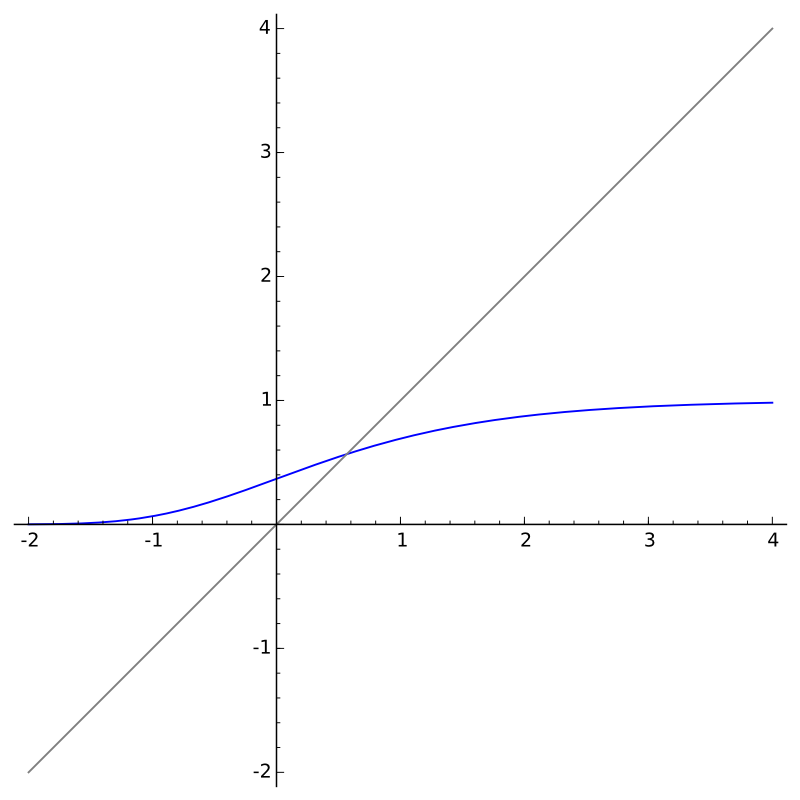
\includegraphics[scale=0.4]{figures/suites-visual2}
\end{center} 

  Cela prouve en particulier que $\ell=\ell'$.


  \item  Par ailleurs la fonction $f$ admet un unique point fixe $x_0$.
  Mais comme $f(x_0)=x_0$ alors l'égalité $f\big( f(x_0) \big) = f\big(x_0\big) = x_0$
  prouve que $x_0$ est aussi le point fixe de $g$.
  
  \item Conclusion : la suite $(u_{2n})$ et la suite $(u_{2n+1})$ convergent
  vers $x_0=\ell=\ell'$. Ainsi la suite $(u_n)$ converge vers $x_0$ le point fixe de $f$.

  
  \item Il n'y a pas d'expression simple de la solution $x_0$ de l'équation $f(x)=x$.
  La commande \codeinline{solve(f(x)==x,x)} renvoie seulement l'équation.
  Par contre, on obtient une valeur numérique approchée par l'instruction 
  \codeinline{find_root(f(x)==x,0,1)}. On trouve $x_0 = 0,56714329041\ldots$
  
\end{enumerate}
\end{enumerate}


%--------------------------------------------------------
\subsection{Listes}

Une \defi{liste} est ce qui ressemble le plus à une suite mathématique.
Une liste est une suite de nombres, de points\ldots ou même de listes !

\begin{itemize}
  
  \item Une liste est présentée entre crochets :
  \codeinline{mesprems = [2,3,5,7,11,13]}. 
  On accède aux valeurs par \codeinline{mesprems[i]} ;
  \codeinline{mesprems[0]} vaut $2$,  \codeinline{mesprems[1]} vaut $3$\ldots
  

  \item On parcourt les éléments d'une liste avec \codeinline{for p in mesprems:}, 
  $p$ vaut alors successivement $2$, $3$, $5$, $7$\ldots
  
  \item Une première façon de créer une liste est de partir de la liste vide, 
  qui s'écrit \codeinline{[]},
  puis d'ajouter un à un des éléments à l'aide de la méthode \codeinline{append}. 
  Par exemple \codeinline{mespoints=[]}, puis \codeinline{mespoints.append((2,3))},
  \codeinline{mespoints.append((7,-1))}. La liste \codeinline{mespoints} contient alors deux
  éléments (c'est-à-dire deux points)  \codeinline{[ (2,3), (7,-1) ]}.

\end{itemize}
  
\begin{tp}
Pour un entier $n$ fixé. Construire : %Composer les listes suivantes :
\begin{enumerate}
  \item la liste des entiers de $0$ à $n-1$,
  
  \item la liste des entiers premiers strictement inférieurs à $n$,
  
  \item la liste des $2p+1$, pour les premiers $p$ strictement inférieurs à $n$,
  
  \item les $10$ premiers éléments de la liste précédente,
    
  \item la liste de $p_i+i$, où $(p_i)_{i\ge0}$ sont les nombres premiers 
  strictement inférieurs à $n$ ($p_0=2$, $p_1=3$,...),
  
  \item la liste de $1$ et $0$ selon que le rang $0\le k <n$ est premier ou non.
\end{enumerate} 
\end{tp}


Une utilisation intelligente permet un code très court et très lisible.
Il faut consulter le manuel pour apprendre à manipuler les listes avec aisance.
\begin{enumerate}
  \item \codeinline{entiers = range(n)}
  \item \codeinline{premiers = [k for k in range(n) if is_prime(k)]} 
  \item \codeinline{doubles = [2*p+1 for p in premiers]}
  \item \codeinline{debut = doubles[0:10]}
  \item \codeinline{premiersplusrang = [premiers[i]+i for i in range(len(premiers))]}
  \item \codeinline{binaire = [zeroun(k) for k in range(n)]} 
  où \codeinline{zeroun(k)} est une fonction à définir qui renvoie $1$ ou $0$ 
  selon que $k$ est premier ou pas. 
\end{enumerate}

On peut aussi trier les listes, les fusionner...

% 
% %--------------------------------------------------------
% \subsection{La constante de Champernowne [à virer ?]}
% 
% Le tp suivant peut être passé lors d'une première lecture.
% 
% \begin{tp}
% La constante de Champernowne
% est 
% $$\tau  = 0,0123456789\ 000102030405060708091011121314\ldots $$
% Les décimales sont formées de tous les nombres à $1$ chiffres ($0,1,2,\ldots,9$), puis tous les nombres
% à $2$ chiffres($00,01,2,\ldots,99$), puis tous les nombres à $3$ chiffres,... 
% 
% \begin{enumerate}
%   \item \'Ecrire une fonction qui renvoie le réels
%   $\tau_k$, dont les décimales sont formées des entiers de $1$ à $k$ chiffres.
%   
%   \item \'Ecrire une fonction qui renvoie la partie fractionnaire $\{x\}$ d'un réel $x$ :
%   $$\{x\} = x - E(x)$$
%   où $E(x)$ désigne la partie entière.
%   
%   \item Soit $x\in \Rr$. Montrer que pour tout $\epsilon>0$, il existe $p$ tel que
%   $$\big| \{x\} - \{10^p \tau\} \big| < \epsilon$$
%  
%  \item Faire le même travail avec la constante binaire de Champernowne, dont l'écriture binaire
%  $$\sigma = 0,\ 0 \ 1 \ 00 \ 01 \ 10 \ 11 \ 000 \ 001 \ 010 \ldots$$
%  formés de la juxtaposition des entiers en écriture binaires à $1$, $2$, $3$,\ldots chiffres.
%  On note $\{x\}_2$ la partie fractionnaire d'un réel en écriture binaire.
%  Montrer que, quelque soit $x\in\Rr$, quelque soit $\epsilon>0$, il existe $p$ tel que
%   $$\big| \{x\}_2 - \{2^p \tau\}_2 \big| < \epsilon$$
% \end{enumerate}
% \end{tp}


%--------------------------------------------------------
\subsection{Suites et chaos}


\begin{tp}
On considère la fonction $f$ définie sur $[0,1]$ par 
$$f(x)=rx(1-x)$$
où $r$ est un réel compris entre $0$ et $4$.

Pour $r$ fixé et $u_0 \in [0,1]$ fixé, on définit une suite $(u_n)$ par
$$u_{n+1} = f(u_n).$$

\begin{enumerate}
  \item Pour différentes valeurs de $r$ et $u_0$ choisies, tracer sur un même graphique
  le graphe de $f$, la droite d'équation $(y=x)$ et quelques termes de la suite $(u_n)$. Essayez de conjecturer 
  le comportement de la suite pour $0<r\le3$, $3< r \le 1+\sqrt{6}$,
  $1+\sqrt{6}< r < 4$ et $r=4$. 
  
  \item Pour $u_0$ fixé et $M<N$ grands (par exemple $M=100$, $N=200$), tracer le \defi{diagramme
  de bifurcation} de $f$, c'est-à-dire l'ensemble des points
  $$(u_i,r) \qquad \text{ pour } \quad M \le i \le N \text{ et } 0 \le r \le 4$$
  
  \item 
  \begin{enumerate}
    \item Montrer que les points fixes de $f$ sont $0$ et $\frac{r-1}{r}$.
    \item Montrer que le point fixe $0$ est répulsif (c'est-à-dire $|f'(0)|>1$) dès que $r>1$.
    \item Montrer que le point fixe $\frac{r-1}{r}$ est attractif (c'est-à-dire $|f'(\frac{r-1}{r})|<1$)
    si et seulement si $1< r < 3$. 
  \end{enumerate}  
  
  
  \item \textbf{Cas $1 < r \le3$. Pour $0<u_0<1$ la suite $(u_n)$ converge vers $\frac{r-1}{r}$.}
 
  Nous allons prouver ce résultat dans le cas particulier $r=2$ :
  \begin{enumerate}
    \item Montrer que $u_{n+1}-\frac12 = -2\left(u_n-\frac12\right)^2$.
    \item Montrer que si $|u_0-\frac12| < k < \frac12$ alors 
    $|u_n-\frac12| < \frac12 (2k)^{2^n}$.
    \item Conclure.
  \end{enumerate} 
  
  \item \textbf{Cas $3<r<1+\sqrt{6}$. La suite $(u_n)$ possède un cycle attracteur de période $2$.}
   
  \begin{enumerate}
    \item Déterminer les points fixes $\ell_1$ et $\ell_2$ de $f\circ f$ qui ne sont pas des points fixes 
    de $f$.
     
    \item Montrer que $f(\ell_1) = \ell_2$ et $f(\ell_2)=\ell_1$.
     
    \item \`A l'aide du graphe de $f\circ f$, vérifier graphiquement sur un exemple, 
    que les suites $(u_{2n})$ et $(u_{2n+1})$ sont croissantes ou décroissantes à partir d'un certain rang
    et convergent, l'une vers $\ell_1$, l'autre vers $\ell_2$.
  \end{enumerate} 
  
  
  \item \textbf{Cas $1+\sqrt{6}<r<3, 5699456\ldots$ La suite $(u_n)$ possède 
  un cycle attracteur de période $4,8,16...$}
  
  Trouver de tels exemples.    
  
  \item \textbf{\`A partir de $r > 3, 5699456\ldots$ la suite $(u_n)$ devient chaotique.}
\end{enumerate}
\end{tp}


%Le tp suivant sera consacré au cas $r=4$.


\begin{enumerate}
  \item 
  Voici le comportement de différentes suites définies par le même $u_0=0,123$ et pour $r$ valant 
  successivement $r=2,2$, $r=3,2$, $r=3,57$ et $r=4$.
  \begin{center}
  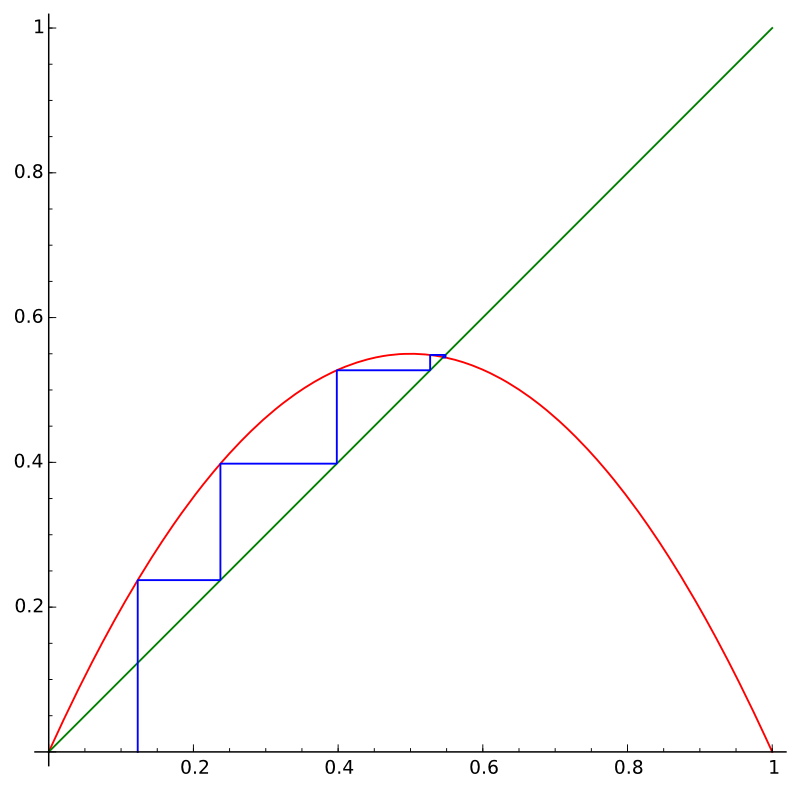
\includegraphics[scale=0.3]{figures/chaos1}\quad
  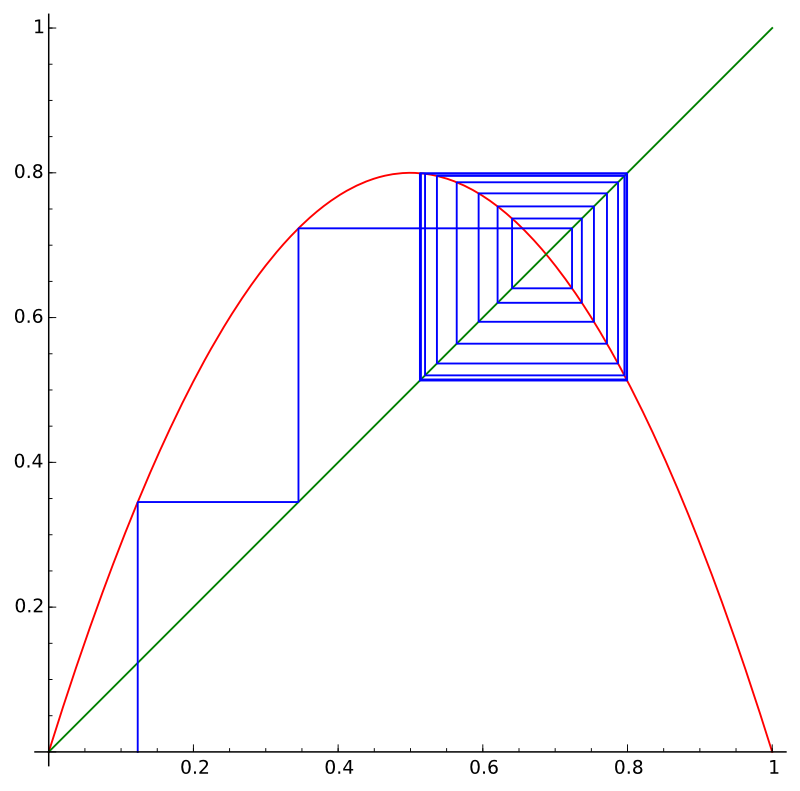
\includegraphics[scale=0.3]{figures/chaos2}\\[3mm]
  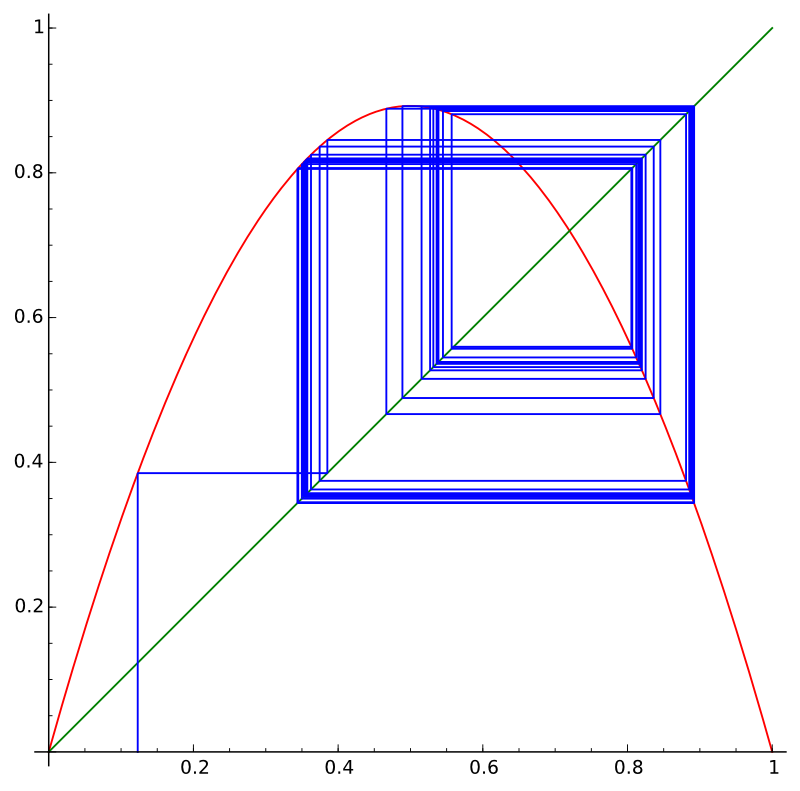
\includegraphics[scale=0.3]{figures/chaos3}\quad
  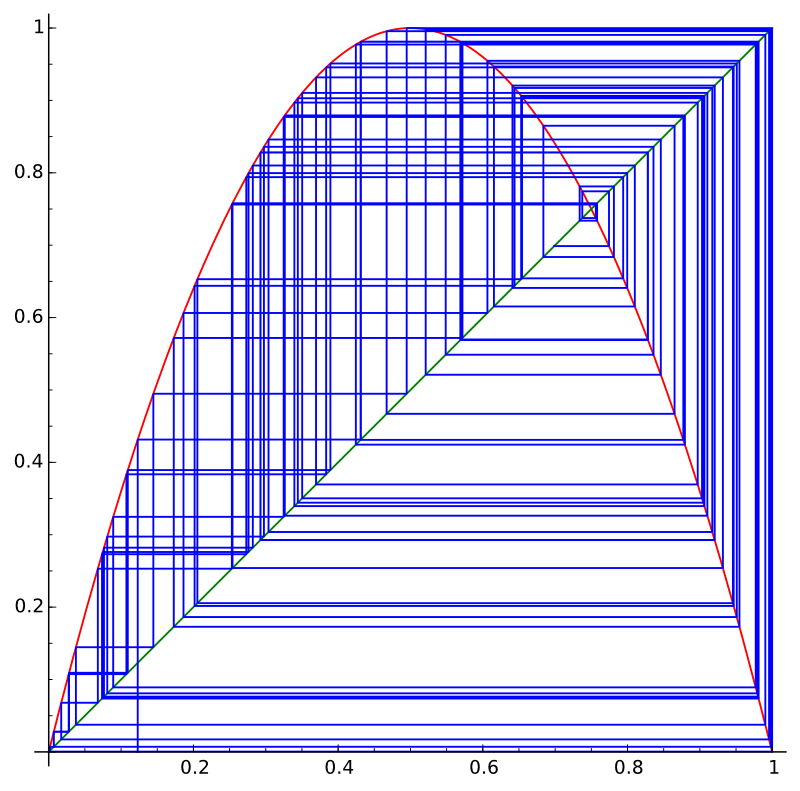
\includegraphics[scale=0.3]{figures/chaos4}  
  \end{center}
  On voit d'abord une limite, puis la suite semble avoir \og deux limites \fg, c'est-à-dire
  deux valeurs d'adhérence, puis $4$ valeurs d'adhérence. Pour 
  $r=4$ la situation semble chaotique.
  
  
  
  \item Voici le code et le résultat de l’exécution \codeinline{bifurcation(f,0.102)},
  où \codeinline{f(x,r) = r*x*(1-x)}.
  
  \insertcode{algos/suites-chaos-tex1.sage}{suites-chaos.sage (1)}
  
  \begin{center}
  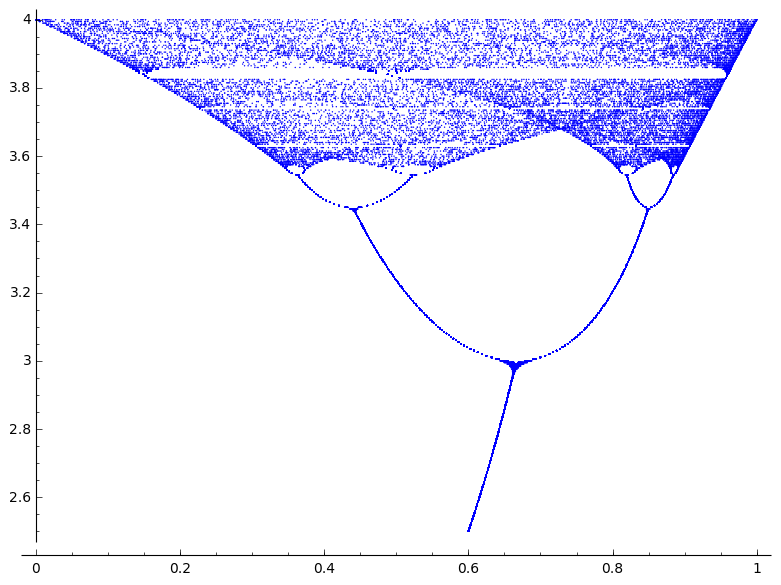
\includegraphics[scale=0.7]{figures/chaos5}  
  \end{center} 

  \item Voici le code pour les trois questions.
    
  \insertcode{algos/suites-chaos-tex2.sage}{suites-chaos.sage (2)}

  
    \begin{enumerate}
    \item Les deux points fixes fournis dans la liste \codeinline{pts_fixes}
    sont $0$ et $\frac{r-1}{r}$. 
    
    \item On calcule la dérivée \codeinline{ff}, 
    on l'évalue en $x=0$, on trouve $f'(0)=r$. Ainsi, si $r>1$ alors
    $|f'(0)|>1$ et le point $0$ est répulsif. 
    
    \item Par contre lorsque l'on résout l'inéquation $|f'(\frac{r-1}{r})|<1$, 
    la machine renvoie les conditions $r>1$ et $r < 3$. 
    Ainsi, pour $1<r<3$, le point fixe $\frac{r-1}{r}$ est attractif.
  \end{enumerate} 
  
  \item On pose d'abord \codeinline{r = 2}, alors le point fixe est $\frac{r-1}{r}= \frac12$.
  \begin{enumerate}
    \item Après simplification \codeinline{(r*u*(1-u) - 1/2) + 2*(u-1/2)^2} vaut $0$.
    Autrement dit $u_{n+1}-\frac12 = -2(u_n-\frac12)^2$, quel que soit $u_n$.
    \item C'est une simple récurrence :
    $$\left|u_{n+1}-\frac12\right|  = 2 \left(u_n-\frac12\right)^2 
    < 2\left(\frac12 (2k)^{2^n}\right)^2 = \frac12 (2k)^{2^{n+1}}.$$
    \item Ainsi pour $u_0 \neq 0,1$, il existe $k$ tel que $|u_0-\frac12| < k < \frac12$
    et la suite $(u_n)$ tend (très très) vite vers le point fixe $\frac12$.
  \end{enumerate} 
  
  Avec $r=2$, en quelques itérations, le terme de la suite 
  n'est plus discernable de la limite $\frac12$ :
  \begin{center}
  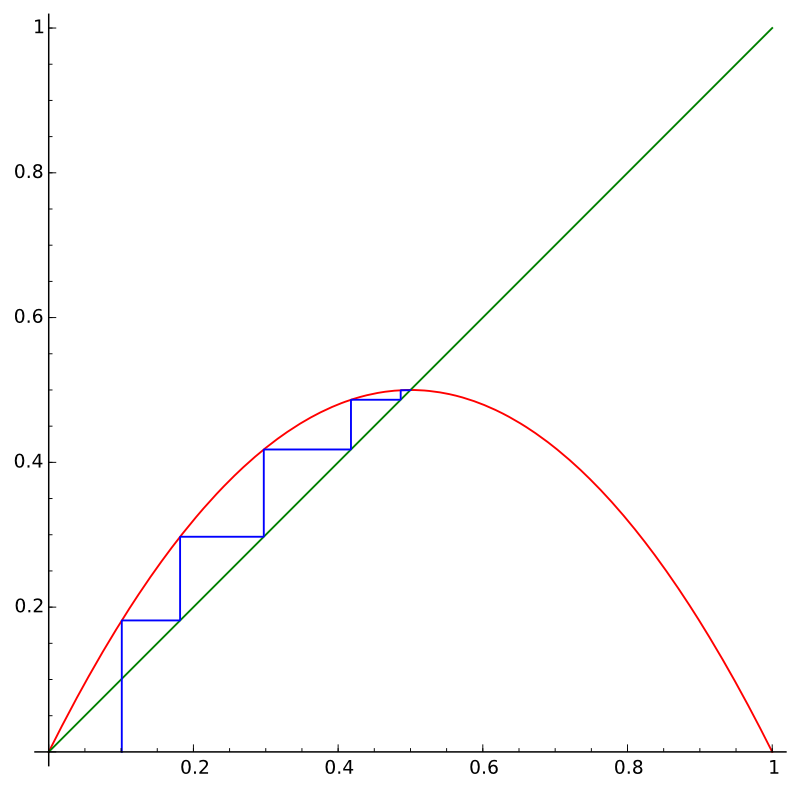
\includegraphics[scale=0.4]{figures/chaos6}  
  \end{center}   
  
  \item  Voici le code pour les deux premières questions :
  
  \insertcode{algos/suites-chaos-tex3.sage}{suites-chaos.sage (3)}

  \begin{enumerate}
    \item On calcule les points fixes de $g = f\circ f$. Il y en a quatre, mais deux d'entre eux sont 
    les points fixes de $f$. Les deux nouveaux sont :
    $$\ell_1 = \frac12\frac{r + 1 - \sqrt{r^2 - 2r - 3}}{r} \qquad \mbox{et} \qquad 
      \ell_2 = \frac12\frac{r + 1 + \sqrt{r^2 - 2r - 3}}{r}.$$
      
    \item Bien sûr, $\ell_1$ et $\ell_2$ ne sont pas des points fixes pour $f$.
    Par contre, on vérifie que $f(\ell_1) = \ell_2$ et $f(\ell_2)=\ell_1$.
     
    \item Voici les dessins pour $r=1+\sqrt{5}$ et $u_0=\frac23$.
    La suite $(u_{2n})$, qui est vue comme suite récurrente de fonction $g$,
    est décroissante vers $\ell_1$ (figure de gauche).
    La suite $(u_{2n+1})$, vue comme suite récurrente de fonction $g$,
    est croissante vers $\ell_2$ (figure de droite).
  \begin{center}
  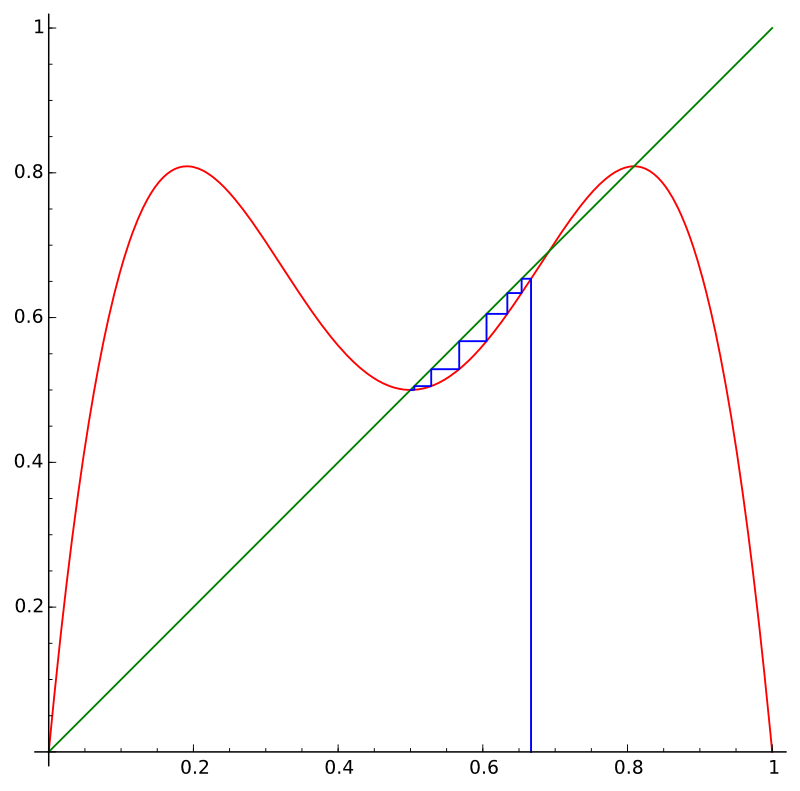
\includegraphics[scale=0.3]{figures/chaos7}\quad
  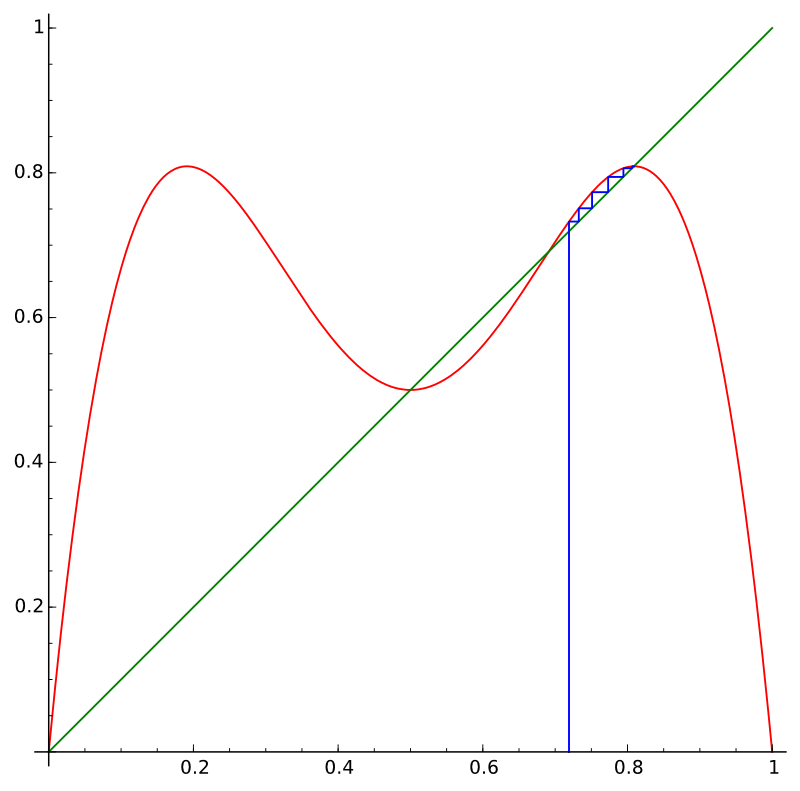
\includegraphics[scale=0.3]{figures/chaos8}
  \end{center}
  
  La suite $(u_n)$, comme suite récurrente de fonction $f$, possède 
  le cycle $(\ell_1,\ell_2)$ comme cycle attracteur :
  \begin{center}
  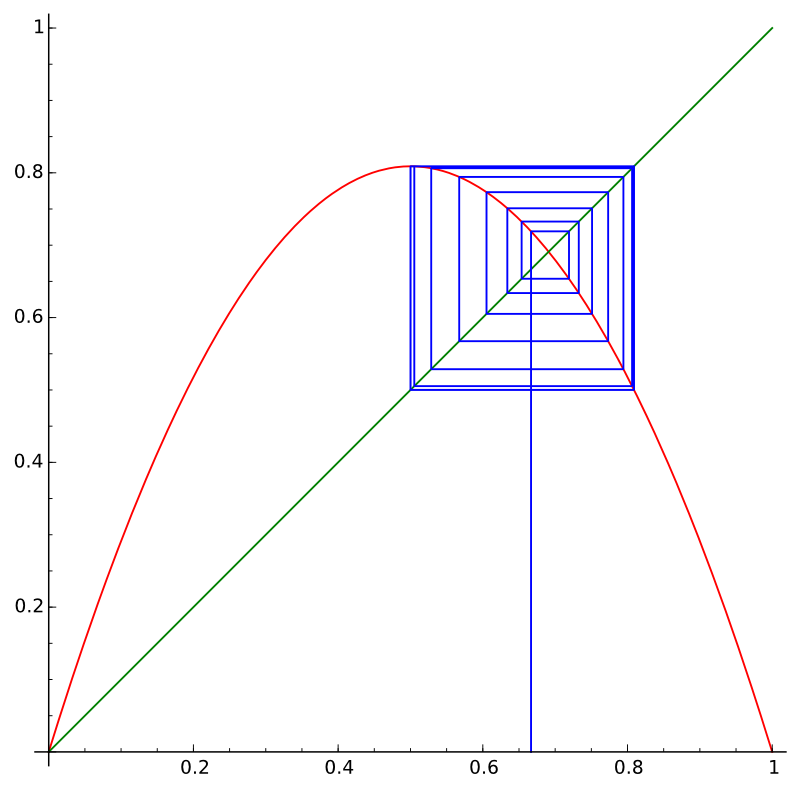
\includegraphics[scale=0.4]{figures/chaos9}
  \end{center}
  \end{enumerate} 
  
  \item Voici un exemple de cycle de longueur $8$ ($r=3,56$, $u_0=0,35$) :
    \begin{center}
  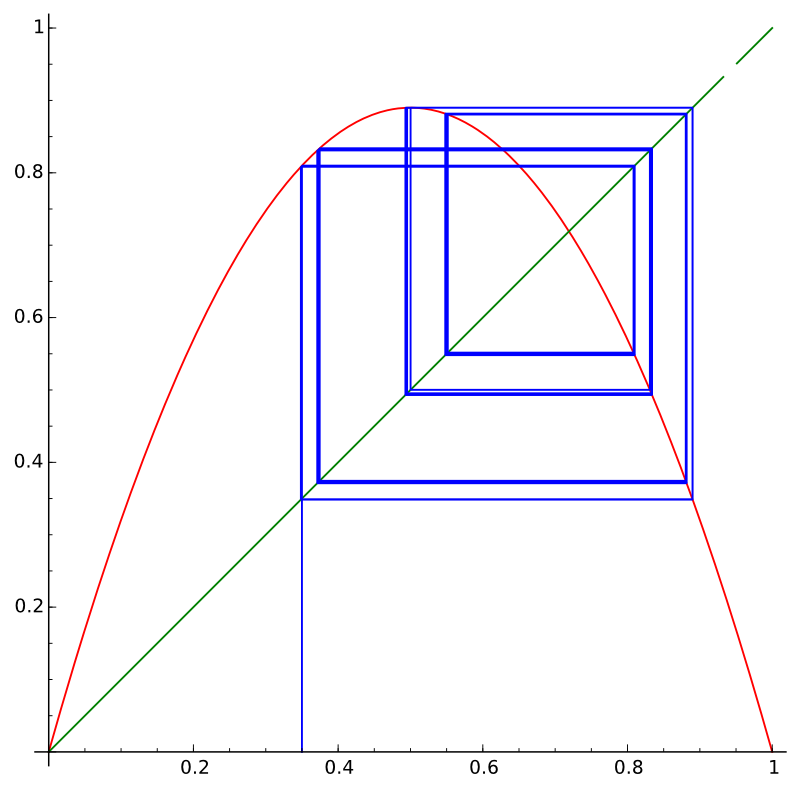
\includegraphics[scale=0.4]{figures/chaos10}
  \end{center}
  
  \item Le cas $r=4$ sera étudié dans le tp suivant.
      
     
\end{enumerate}


\begin{tp}
On s'intéresse au cas $r=4$. On rappelle que 
$$f(x)=rx(1-x)$$
et que 
$$u_0 \in [0,1] \qquad \mbox{et} \qquad u_{n+1} = f(u_n)\quad (n\geq 0).$$

\begin{enumerate}
  \item 
  \begin{enumerate}
    \item Montrer que $\sin^2(2t) = 4 \sin^2 t \cdot (1-\sin^2 t)$.
    \item Montrer que pour $u_0 \in [0,1]$, il existe un unique $t \in [0,\frac\pi2]$ tel que
    $u_0 = \sin^2 t$.
    \item En déduire $u_n = \sin^2(2^n t)$.
  \end{enumerate}
  
  \item Pour $t_k = \frac{2\pi}{2^k+1}$ et $u_0 = \sin^2 t_k$, 
  montrer que la suite $(u_n)$ est périodique de période $k$.
  
  \item \textbf{La suite est instable.}
  \begin{enumerate}
    \item Pour $k=3$, on pose $t_3 = \frac{2\pi}{9}$ et $u_0 = \sin^2 t_3$.
    Calculer une valeur exacte (puis approchée) de $u_n$, pour différentes valeurs de $n$.
    
    \item Partant d'une valeur approchée $\tilde{u}_0$ de $u_0$, 
    que donne la suite des approximations $(\tilde{u}_n)$ définie 
    par la relation de récurrence ?
  \end{enumerate}
  
    
  \item \textbf{La suite est partout dense.}
  
  On va construire $u_0\in[0,1]$ tel que, tout $x\in[0,1]$ peut être approché d'aussi près que l'on veut par 
  un terme $u_n$ de notre suite :
  $$\forall x \in [0,1] \quad \forall \epsilon > 0 \quad \exists n \in \Nn \qquad \big| x -u_n \big| < \epsilon.$$
  
  
  \begin{itemize}
    \item Soit $\sigma$ la constante binaire de Champernowne, 
    formée de la juxtaposition des entiers en écriture binaire 
    à $1$, $2$, $3$,\ldots chiffres $0$, $1$, $00$, $01$, $10$,...
    dont l'écriture binaire est $\sigma = 0,0100011011\ldots$
    
    \item Soit $u_0 = \sin^2 (\pi\sigma)$. 
    
    \item Soit $x \in [0,1[$. Ce réel peut s'écrire $x = \sin^2(\pi t)$ avec 
    $t\in [0,1[$ qui admet une écriture binaire $t= 0,a_1 a_2 \ldots a_p \ldots$.
  \end{itemize}
  
  Pour $\epsilon>0$ fixé, montrer qu'il existe $n$ tel que $\big| x -u_n \big| < \epsilon$.
  
\end{enumerate}

\end{tp}

\begin{enumerate}
  \item 
  \begin{enumerate}
    \item On pose \codeinline{eq = sin(2*t)^2 - 4*sin(t)^2*(1-sin(t)^2)}
    et \codeinline{eq.full_simplify()} renvoie $0$. Donc 
    $\sin^2(2t) = 4 \sin^2 t \cdot (1-\sin^2 t)$, pour tout $t\in\Rr$.
    
    \item Soit $h(t) = \sin^2 t$. On définit la fonction \codeinline{h = sin(t)^2}, sa dérivée 
    \codeinline{hh = diff(h,t)} dont on cherche les zéros 
    par \codeinline{solve(hh==0,t)}. La dérivée ne s'annulant qu'en $t=0$ et
    $t=\frac\pi2$, la fonction $h'$ est strictement monotone sur $[0,\frac\pi2]$.
    Comme $h(0)=0$ et $h(\frac\pi2)=1$, pour chaque $u_0 \in [0,1]$, 
    il existe un unique $t \in [0,\frac\pi2]$ tel que
    $u_0 = h(t)$. 
    \item Pour $u_0 = \sin^2 t$, on a 
    $$u_{1} = f(u_0) = ru_0(1-u_0) = 4\sin^2 t \cdot (1-\sin^2 t) =  \sin^2(2 t).$$
    On montre de même par récurrence que $u_n =   \sin^2(2^n t)$.
  \end{enumerate}
  
  \item Le code suivant calcule $u_k-u_0$.
  \Sage\ sait calculer que cela vaut $0$, pour $k$ prenant la valeur $0$, $1$, $2$,...
  mais pas lorsque $k$ est une variable. Le calcul à la main est pourtant très simple !
  
    \insertcode{algos/suites-chaos-tex4.sage}{suites-chaos.sage (4)}
 
  \item \textbf{La suite est instable.}
  \begin{enumerate}
    \item  Pour $k=3$ et $t_3 = \frac{2\pi}{9}$, la suite $(u_k)$ est périodique de période $3$.
    Il suffit donc de calculer $u_0,u_1,u_2$.
    Par exemple :
    $$u_{3p} = u_0 = \sin^2\left( \frac{2\pi}{9}\right) \simeq \num{0.4131759111\dots}$$
    
    \item Partons de la valeur approchée de $u_0$ avec $10$ décimales exactes :    
    $\tilde{u}_0 = \num{0.4131759111}$ et calculons les premiers termes de la suite. On en extrait :

\begin{center}
\setlength{\arrayrulewidth}{0.05mm}
\begin{tabular}{c} 
%\begin{tabular}[t]{cc@{\vrule depth 2.5ex height 3.5ex width 0mm \ }} 
$\tilde{u}_0\simeq $    \num{0.413175911100} \\
$\tilde{u}_3\simeq $    \num{0.413175911698} \\
$\tilde{u}_6\simeq $    \num{0.413175906908} \\
$\tilde{u}_9\simeq $    \num{0.413175945232} \\
$\tilde{u}_{12}\simeq $ \num{0.413175638640} \\
$\tilde{u}_{15}\simeq $ \num{0.413178091373} \\
$\tilde{u}_{18}\simeq $ \num{0.413158469568} \\
$\tilde{u}_{21}\simeq $ \num{0.413315447870} \\
$\tilde{u}_{24}\simeq $ \num{0.412059869464} \\
$\tilde{u}_{27}\simeq $ \num{0.422119825829} \\
$\tilde{u}_{30}\simeq $ \num{0.342897499745} \\
$\tilde{u}_{33}\simeq $ \num{0.916955513784} \\
$\tilde{u}_{36}\simeq $ \num{0.517632311613} \\
$\tilde{u}_{39}\simeq $ \num{0.019774022431} \\
\end{tabular} 
\end{center} 

Si l'approximation de départ et tous les calculs étaient exacts, on devrait obtenir
$u_0$ à chaque ligne. On constate que l'erreur augmente terme après terme, 
et après $\tilde{u}_{30}$, le comportement de $\tilde{u}_{n}$ 
n'a plus rien à voir avec $u_n$.
L'explication vient de la formule $u_n =   \sin^2(2^n t)$, une erreur 
sur $t$, même infime au départ, devient grande par multiplication par $2^n$.

  \end{enumerate}
  
    
  \item \textbf{La suite est partout dense.}
  
  La construction est assez jolie mais délicate. (Il ne faut pas avoir peur de 
  l'écriture en base $2$ qui n'est pas ici le point clé. 
  Vous pouvez penser en base $10$ pour mieux comprendre.)
  
  
  Fixons $\epsilon >0$. Soit un entier $p$ tel que 
  $\frac{\pi}{2^p} < \epsilon$.
  L'écriture binaire de $t$ étant $t= 0,a_1 a_2 \ldots a_p \ldots$
  la séquence $a_1 a_2 \ldots a_p$ apparaît quelque part dans la constante de
  Champernowne. Plus précisément, il existe un entier $n$ tel que
  $2^n \sigma = \ldots b_2b_1b_0,a_1 a_2 \ldots a_p\ldots$
  (on a fait apparaître la séquence juste après la virgule par 
  décalage de la virgule).
  
  On va pouvoir oublier la partie entière $m = \ldots b_2b_1b_0 \in \Nn$ et on note $\tilde \sigma 
  = 0,a_1 a_2 \ldots a_p\ldots$ la partie fractionnaire de $\sigma$, 
  de sorte que $2^n \sigma = m + \tilde  \sigma$.
  
  \begin{align*}
  |x-u_n| 
    &= \left| \sin^2(\pi t) - \sin^2(2^n \pi \sigma)\right| \\
   &= \left| \sin^2(\pi t) - \sin^2(2^n \pi m + \pi \tilde\sigma)\right| \\ 
    &=   \left| \sin^2(\pi t) - \sin^2(\pi \tilde\sigma)\right| 
      \qquad \text{ car $\sin^2$ est $\pi$-périodique}\\
    &\le  \left| \pi t - \pi \tilde\sigma\right| 
      \qquad \text{ par le théorème des accroissements finis}\\
    &\le  \pi \frac1{2^p}  
      \qquad \text{ car $t$ et $\tilde\sigma$ ont les mêmes $p$ premières décimales}\\
    &< \epsilon
  \end{align*}

  Conclusion : n'importe quel $x$ est approché d'aussi près que 
  l'on veut par la suite. 
  
\end{enumerate}


\bigskip

Pour en savoir plus : 
\begin{itemize}
  \item \href{http://www.math.u-psud.fr/~perrin/Conferences/logistiqueDP.pdf}
  {\emph{La suite logistique et le chaos}}, Daniel Perrin.
  
  \item %\href{http://www.casio-education.fr/calculatrice_casio_documents/exercices/classpad330/exo001.pdf}
  {\emph{\'Etude d’une suite récurrente}}, Jean-Michel Ferrard.
\end{itemize}

\finchapitre
\end{document}

